\vspace{-1.2em}
\section{Deep Parameter Optimisation}
\label{sec_deep_parameter_optimisation}

Figure~\ref{system} shows the work flow of our deep parameter optimisation. The approach takes the source code of the program, a set of test data and a set of non-functional properties of interest. 
It first applies mutation analysis and a non-dominated rank algorithm to discover potential locations for deep parameters, as explained in Section~\ref{discovering}. It then exposes deep parameters based on the type of expressions found at the locations (Section~\ref{exposing}). Finally, to tune the program, a multi-objective search algorithm is used to search for optimised values for both shallow and deep parameters (Section~\ref{sec_nsgaii}).

\begin{figure}[htbp]
\centering
\vspace{-0.5em}
\scalebox{0.55}{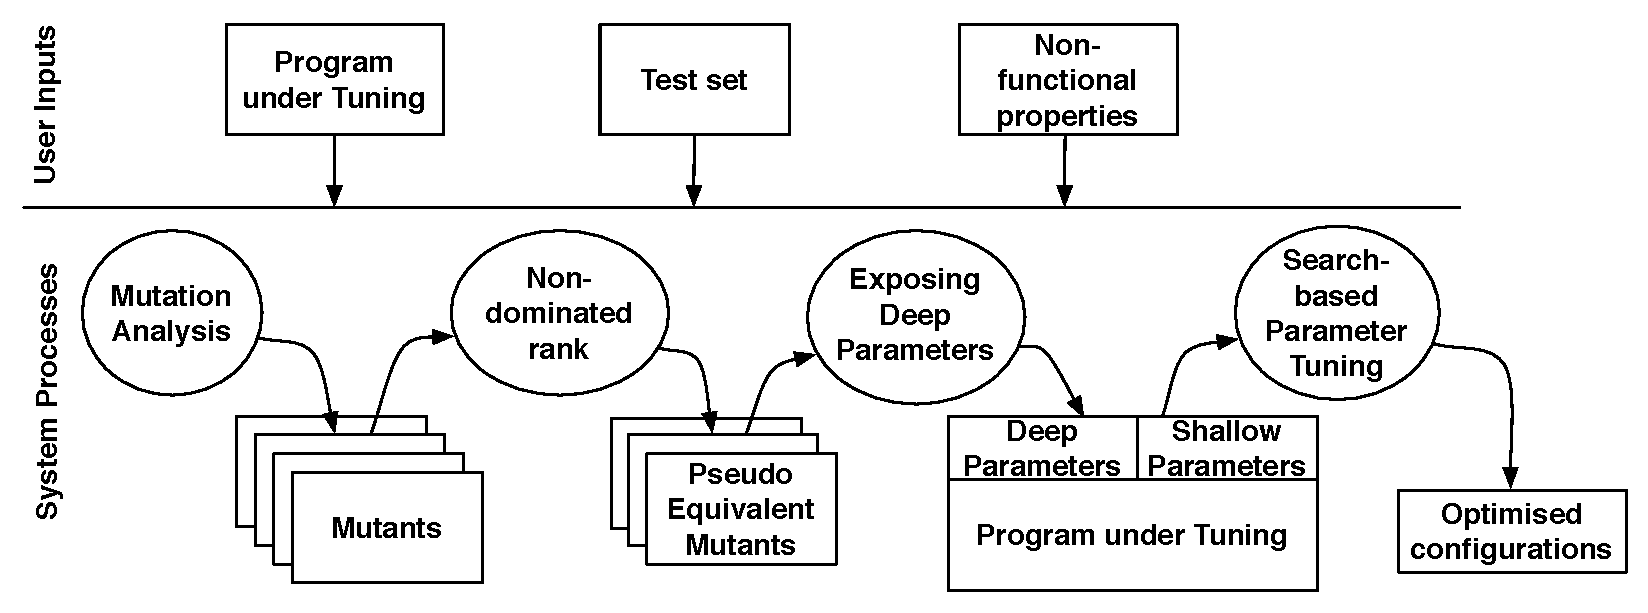
\includegraphics[width=6.2in]{pics/new_system}}
\vspace{-1.8em}
\caption{Deep parameter optimisation workflow. Given a program, test suite and non-functional properties, our approach applies mutation analysis, exposes deep parameters, and optimises them.}\label{system}
\vspace{-1.9em}
\end{figure}

\subsection{Discovering Locations for Deep Parameters}
\label{discovering}
The first step is to identify potential locations at which we could expose deep parameters. 
In our approach, we represent the input program as an Abstract Syntax Tree (AST) and a potential location $L$ is an expression node of the AST. 
We want to find a set of locations $L_D$ such that, when we tune the value of the expression at $L_D$, some non-functional properties of the program could be improved while the program retains identical functional behaviour.
%We use software testing to valid the functional behaviour of the program. 
%To valid the functional behaviour of the tuned program, we test the tuned program with the input test set and compare the output with the test output of the original program.
We use a suite of regression test data to validate the correctness from the optimisation, following other established Genetic Improvement approaches~\cite{babelPidgin,Langdon:2014:IMI:2576768.2598244,justyna2013}. We assume the presence of a test suite with each target application.

We use mutation analysis to automate the process of searching for locations
$L_D$. Mutation analysis deliberately makes simple syntactic changes to the
input program, to create a set of various versions of a program called mutants,
each containing a different syntactic change~\cite{5487526}. A
transformation rule that generates a mutant from the input program is known
as a mutation operator. By carefully choosing mutation operators, we can
use mutants to simulate the effect of making changes at those locations $L$s
from which a potential deep parameter may be exposed. 
% FIXME: Wes does not understand what "simulate the effects of making
% changes at _all_ protential locations" means in the previous sentence.
% Please clarify for the reader. 
% Fan tried to say that, using Mutation Operators, we can simulate
% changes to those locations from which a deep parameter may be exposed,
% thus to aid selecting most sensitive locations.
Table~\ref{tab:cmop} lists the operators we used to generate
mutants, covering locations of constants, relational, logical and
arithmetic expressions. 
% FIXME: Walk us through two operators chosen from tab:comp. Why are they
% good? Why did you pick them? Are they just like MOTHRA? This is a
% contribution of your paper. Elaborate!
% Yue added the following sentence.
These so-called `selective' mutation operators
have been widely used in mutation analysis experiments~\cite{5487526}.

\iffalse
\begin{table*} [ht]
\caption{Selected mutation operators}
\label{tab:cmop} 
\begin{center}
\begin{tabular}{ | c | l | l |}
  \hline
  Mutation Operators & Brief Description & Details \\ 
\hline
  CRCR & Required constant replacement & Replace a scalar reference with constants $0$, $1$, $-1$ \\
  OAAN & Arithmetic operator mutation & Replace \texttt{+}, \texttt{-}, \texttt{*}, \texttt{/}, \texttt{\%} with each other \\
  OAAA & Arithmetic assignment mutation & Replace \texttt{+=}, \texttt{-=}, \texttt{*=}, \texttt{/=}, \texttt{\%=} with each other \\
  OCNG & Logical context negation & Replace \textit{expr} with \texttt{!}\textit{expr} in selective and iterative statements\\
  OIDO & Increment/decrement mutation  & Replace \texttt{++}x, \texttt{--}x, x\texttt{++}, x\texttt{--} with each other \\
  OLLN & Logical operator mutation  & Replace \texttt{\&\&}, \texttt{||} with each other \\ 
  OLNG & Logical negation & Replace $x$ \texttt{op} $y$ with $x$ \texttt{op} \texttt{!}$y$, \texttt{!}$x$ \texttt{op} $y$, \texttt{!}($x$ \texttt{op} $y$)\\
  ORRN & Relational operator mutation & Replace \texttt{>}, \texttt{>=}, \texttt{<}, \texttt{<=}, \texttt{==} with each other \\
  OBBA & Bitwise assignment mutation & Replace \texttt{\&=}, \texttt{|=} with each other \\
  OBBN & Bitwise operator mutation & Replace \texttt{\&}, \texttt{|} with each other \\
\hline
\end{tabular} 
\end{center} 
\end{table*} 
\fi

\begin{table}[t]
\caption{Selected mutation operators}
\label{tab:cmop} 
\begin{center}
\begin{tabular}{ | l | l |}
  \hline
  Mutation Operators & Changes Between \\ 
\hline
 CRCR -- Constant replacement & constants, $0$, $1$, $-1$ \\
 OAAN -- Arithmetic operator & \texttt{+}, \texttt{-}, \texttt{*}, \texttt{/}, \texttt{\%} \\
 OAAA -- Arithmetic assignment & \texttt{+=}, \texttt{-=}, \texttt{*=}, \texttt{/=}, \texttt{\%=} \\
 OCNG -- Logical context negation & \textit{expr}, \texttt{!}\textit{expr} \\
 OIDO -- Increment/decrement & \texttt{++}x, \texttt{{-}-}x, x\texttt{++}, x\texttt{{-}-} \\
  OLLN -- Logical operator & \texttt{\&\&}, \texttt{||} \\ 
  OLNG -- Logical negation & $x$ \texttt{op} $y$, $x$ \texttt{op} \texttt{!}$y$,
  \\
  & \texttt{!}$x$ \texttt{op} $y$, \texttt{!}($x$ \texttt{op} $y$)\\
  ORRN -- Relational operator & \texttt{>}, \texttt{>=}, \texttt{<}, \texttt{<=}, \texttt{==} \\
  OBBA -- Bitwise assignment & \texttt{\&=}, \texttt{|=} \\
  OBBN -- Bitwise operator & \texttt{\&}, \texttt{|} \\
\hline
\end{tabular} 
\vspace*{-9mm}
\end{center} 
\end{table} 

To assess the quality of a mutant, we test each mutant against the input test set and record the values of the non-functional properties. If the functional result of running a mutant is different from the result of running the original program for any test data in the input test set, then the mutant is said to be `killed', otherwise it is said to have `survived'. 
After all mutants are executed, we first filter out the killed mutants
which fail to retain the functional behaviour. A mutant is called
\textbf{pseudo equivalent} with respect to a given test suite $T$ iff. it
passes the regression test of $T$.  Thus we only select pseudo equivalent
mutants which preserve the functional behaviour of the original program
while potentially changing non-functional behaviour. 

In practice, there is a large number of pseudo equivalent mutants~\cite{ MikeEQ2015,weimerGPEM14, Yao:2014:SES:2568225.2568265} generated. We desire a subset from them that represents the locations that could have the greatest impact on the non-functional properties of interest while also maintaining a diversity of choices.  
We achieve this by ranking the mutants based on their non-functional properties using the non-dominated sorting approach of the NSGA-II algorithm~\cite{996017}. Each mutant is assigned a Pareto Level value and a Crowd Distance value, where Pareto Level $n$ means a mutant will be on the Pareto Front after all the mutants with Pareto Level less than $n$ are removed, while Crowd Distance indicates how close a mutant is to its neighbours on the same Pareto Level. For example, a mutant with Pareto Level $1$ is on the Pareto Front among all the mutants and has the priority to be considered first. A mutant is better than another in terms of non-dominated sorting if its Pareto Level is smaller or if their Pareto Levels are the same but the former is less crowded (larger Crowd Distance) than the latter. After sorting all the mutants in terms of their non-functional properties, we apply a greedy algorithm to pick the first $k$ locations that could best influence the non-functional properties of the original, where $k$ is the desired number of deep parameters one wants to expose.
\vspace{-0.8em}
\subsection{Exposing Deep Parameters}
\label{exposing}
The second step is to expose deep parameters that allow users to modify the value of the expression at selected locations. Based on the type of mutation, we first classify the selected mutants into two sets. Set 1 contains mutants generated from CRCR, OAAN, OAAA and OIDO operators, which simulate locations with non-logical expressions. Set 2 contains mutants generated from the OCNG, OLLN, OLNG and ORRN operators, which simulate locations with logical expressions (Table~\ref{tab:cmop}). 
Given a location $L$, $E_L$ is the expression at the location $L$, we use the following transformation rules to rewrite $E_L$ with a new parameter $v_L$.
\vspace{-0.2em}
\begin{equation}
 E_L \rightarrow \left\{
  \begin{array}{l l}
    (E_L + v_L) & \quad \text{if $L$ $\in$ Set 1}\\
    (E_L) \ xor \ v_L & \quad \text{if $L$ $\in$ Set 2}
    \end{array} \right.
\end{equation}

We use addition to affect the value of non-logical expression and \texttt{exclusive or} to affect the logical ones.
Finally we expose $v_L$ as a `public' parameter so that users can assign a value to $v_L$ through parameter passing or APIs.
\vspace{-0.2em}
\subsection{Search-based Parameter Tuning}
\label{sec_nsgaii}

Although the exposed deep parameters can provide additional `knobs'~\cite{Hoffmann:2011:DKR:1950365.1950390} to tune the program, a set of $k$ deep parameters need not necessarily subsume the existing shallow parameters of the program.  Thus, in this work, we propose to use both shallow parameters and deep parameters and tune them together using SBSE~\cite{Harman:2007:CSF:1253532.1254729}. Because we are interested in multiple conflicting properties, we consider this as a multi-objective optimisation problem, thus a multi-objective Genetic Algorithm, NSGA-II~\cite{996017}, is applied to search for optimal values for both shallow and deep parameters.
% FIXME: You introduced NSGA-II in the previous subsection. Don't
% re-introduce it here! 
% Fan thinks this is details of chromosome representation and configuration for NSGA-II we used.

We use an integer vector to represent the tuning parameters. Each integer stores a solution value for one parameter. At each generation, our NSGA-II implementation first applies tournament selection, followed by a uniform crossover and a uniform mutation operation. In our experiments our fitness functions are designed to capture two non-functional properties: execution time and memory consumption, while preserving the functionality by assigning the worst value to both non-functional properties. To measure execution time, \emph{Glibc}'s \emph{wait4} system call is used to calculate the CPU time (mean of 10 evaluations). For memory consumption, we instrumented the program to record the high-water mark of the virtual memory consumption. We chose this instrumentation approach because the physical memory reported by the OS is not always deterministic but depends on the workload and the OS, and because the virtual memory requirement is an upper bound of the physical memory actually needed. For a subject program with configuration $c$, we measure the execution time $t_i(c)$ and the high-water-mark of memory consumption $m_i(c)$ of each test case $i$. Then the fitness functions for the configuration $c$ regarding execution time and memory consumption can be formulated as:
$$f_t(c)=\sum_{i} t_i(c) ~~~~~~~~~~f_m(c)=\sum_{i} m_i(c).$$
After fitness evaluation, a standard NSGA-II non-dominated selection creates the next generation. Finally, all non-dominating solutions in the final population are returned.
